\section{Appendix}
\subsection{Naming Clarification}
\label{appendix:naming_clarification}
Importantly, we clarify that the naming of ‘\textit{encoder}' and `\textit{decoder}' are based on their output characteristics---i.e., the encoder outputs the latent while the decoder outputs the target---rather than being strictly tied to the transformer architecture they utilize. 
For instance, in the encoder-decoder model, the decoder consists of multiple transformer layers with self-attention (referred to as Transformer Encoder layers in the original transformer paper). However, we designate it as a decoder because its primary function is to output results.
These terminologies align with conventions used in LLMs~\citep{vaswani2017transformer, radford2019language, devlin2018bert}.
Notably, we apply self-attention to all tokens in every transformer block of both models without introducing special attention masks or other architectural biases, in line with our philosophy of minimizing inductive bias.

\subsection{Additional Implementation Details}
\label{appendix:more_details}
We train \paperName{} with 64 A100 GPUs with a batch size of 8 per GPU. We use a cosine learning rate schedule with a peak learning rate of $4\text{e-}4$ and a warmup of 2500 iterations. We train \paperName{} for 80k iterations on the object and 100k on scene data. \paperName{} uses a image patch size of $p=8$ and token dimension $d=768$. The details of the transformer layers follow GS-LRM\citep{zhang2024gslrmlargereconstructionmodel} with an additional QK-Norm. 
Unless noted, all models have 24 transformer layers, the same as GS-LRM. The \textit{encoder-decoder} \paperName{} has $12$ encoder layers and $12$ decoder layers, with $3072$ latent tokens. Note that our model size is smaller than GS-LRM, as GS-LRM uses a token dimension of $1024$.

For object-level experiments, we use 4 input views and 8 target views for each training example by default. We first train with a resolution of $256$, which takes 4 days for the \textit{encoder-decoder} model and 7 days for the \textit{decoder-only} model. Then, we finetune the model with a resolution of $512$ for 10k iterations with a smaller learning rate of $4\text{e-}5$ and a smaller total batch size of 128, which takes 2.5 days. For scene-level experiments
We use 2 input views and 6 target views for each training example.  We first train with a resolution of $256$, which takes about 3 days for both \textit{encoder-decoder} and \textit{decoder-only} models. Then, we finetune the model with a resolution of $512$ for 20k iterations with a smaller learning rate of $1\text{e-}4$ and a total batch size of 128 for 3 days.
For both object and scene-level experiments, the view selection details and camera pose normalization methods follow GS-LRM. We use a perceptual loss weight $\lambda$ as 0.5 and 1.0 on scene-level and object-level experiments, respectively.


We do not use bias terms in our model, for both Linear and LayerNorm layers. We initialize the model weights with a normal distribution of zero-mean and standard deviation of $0.02 / (2 * (\textit{idx} + 1)) ** 0.5$, where $\textit{idx}$ means transform layer index.

We train our model with AdamW optimizer~\citep{kingma2014adam}. The $\beta_1$ and $\beta_2$ are set to 0.9 and 0.95 respectively, following GS-LRM. We use a weight decay of 0.05 on all parameters except the weights of LayerNorm layers.

% \newpage

\subsection{Additional Visual Results}
We show the visualization of \paperName{} at the object level with $256$ resolution in Fig.~\ref{fig:lowres_obj}. Consistent with the findings of the experiment with $512$ resolution (Fig.~\ref{fig:highres_obj}), \paperName{} performs better than the baselines on texture details, specular material, and concave geometry. 

\begin{figure}[htp!]
    \centering
    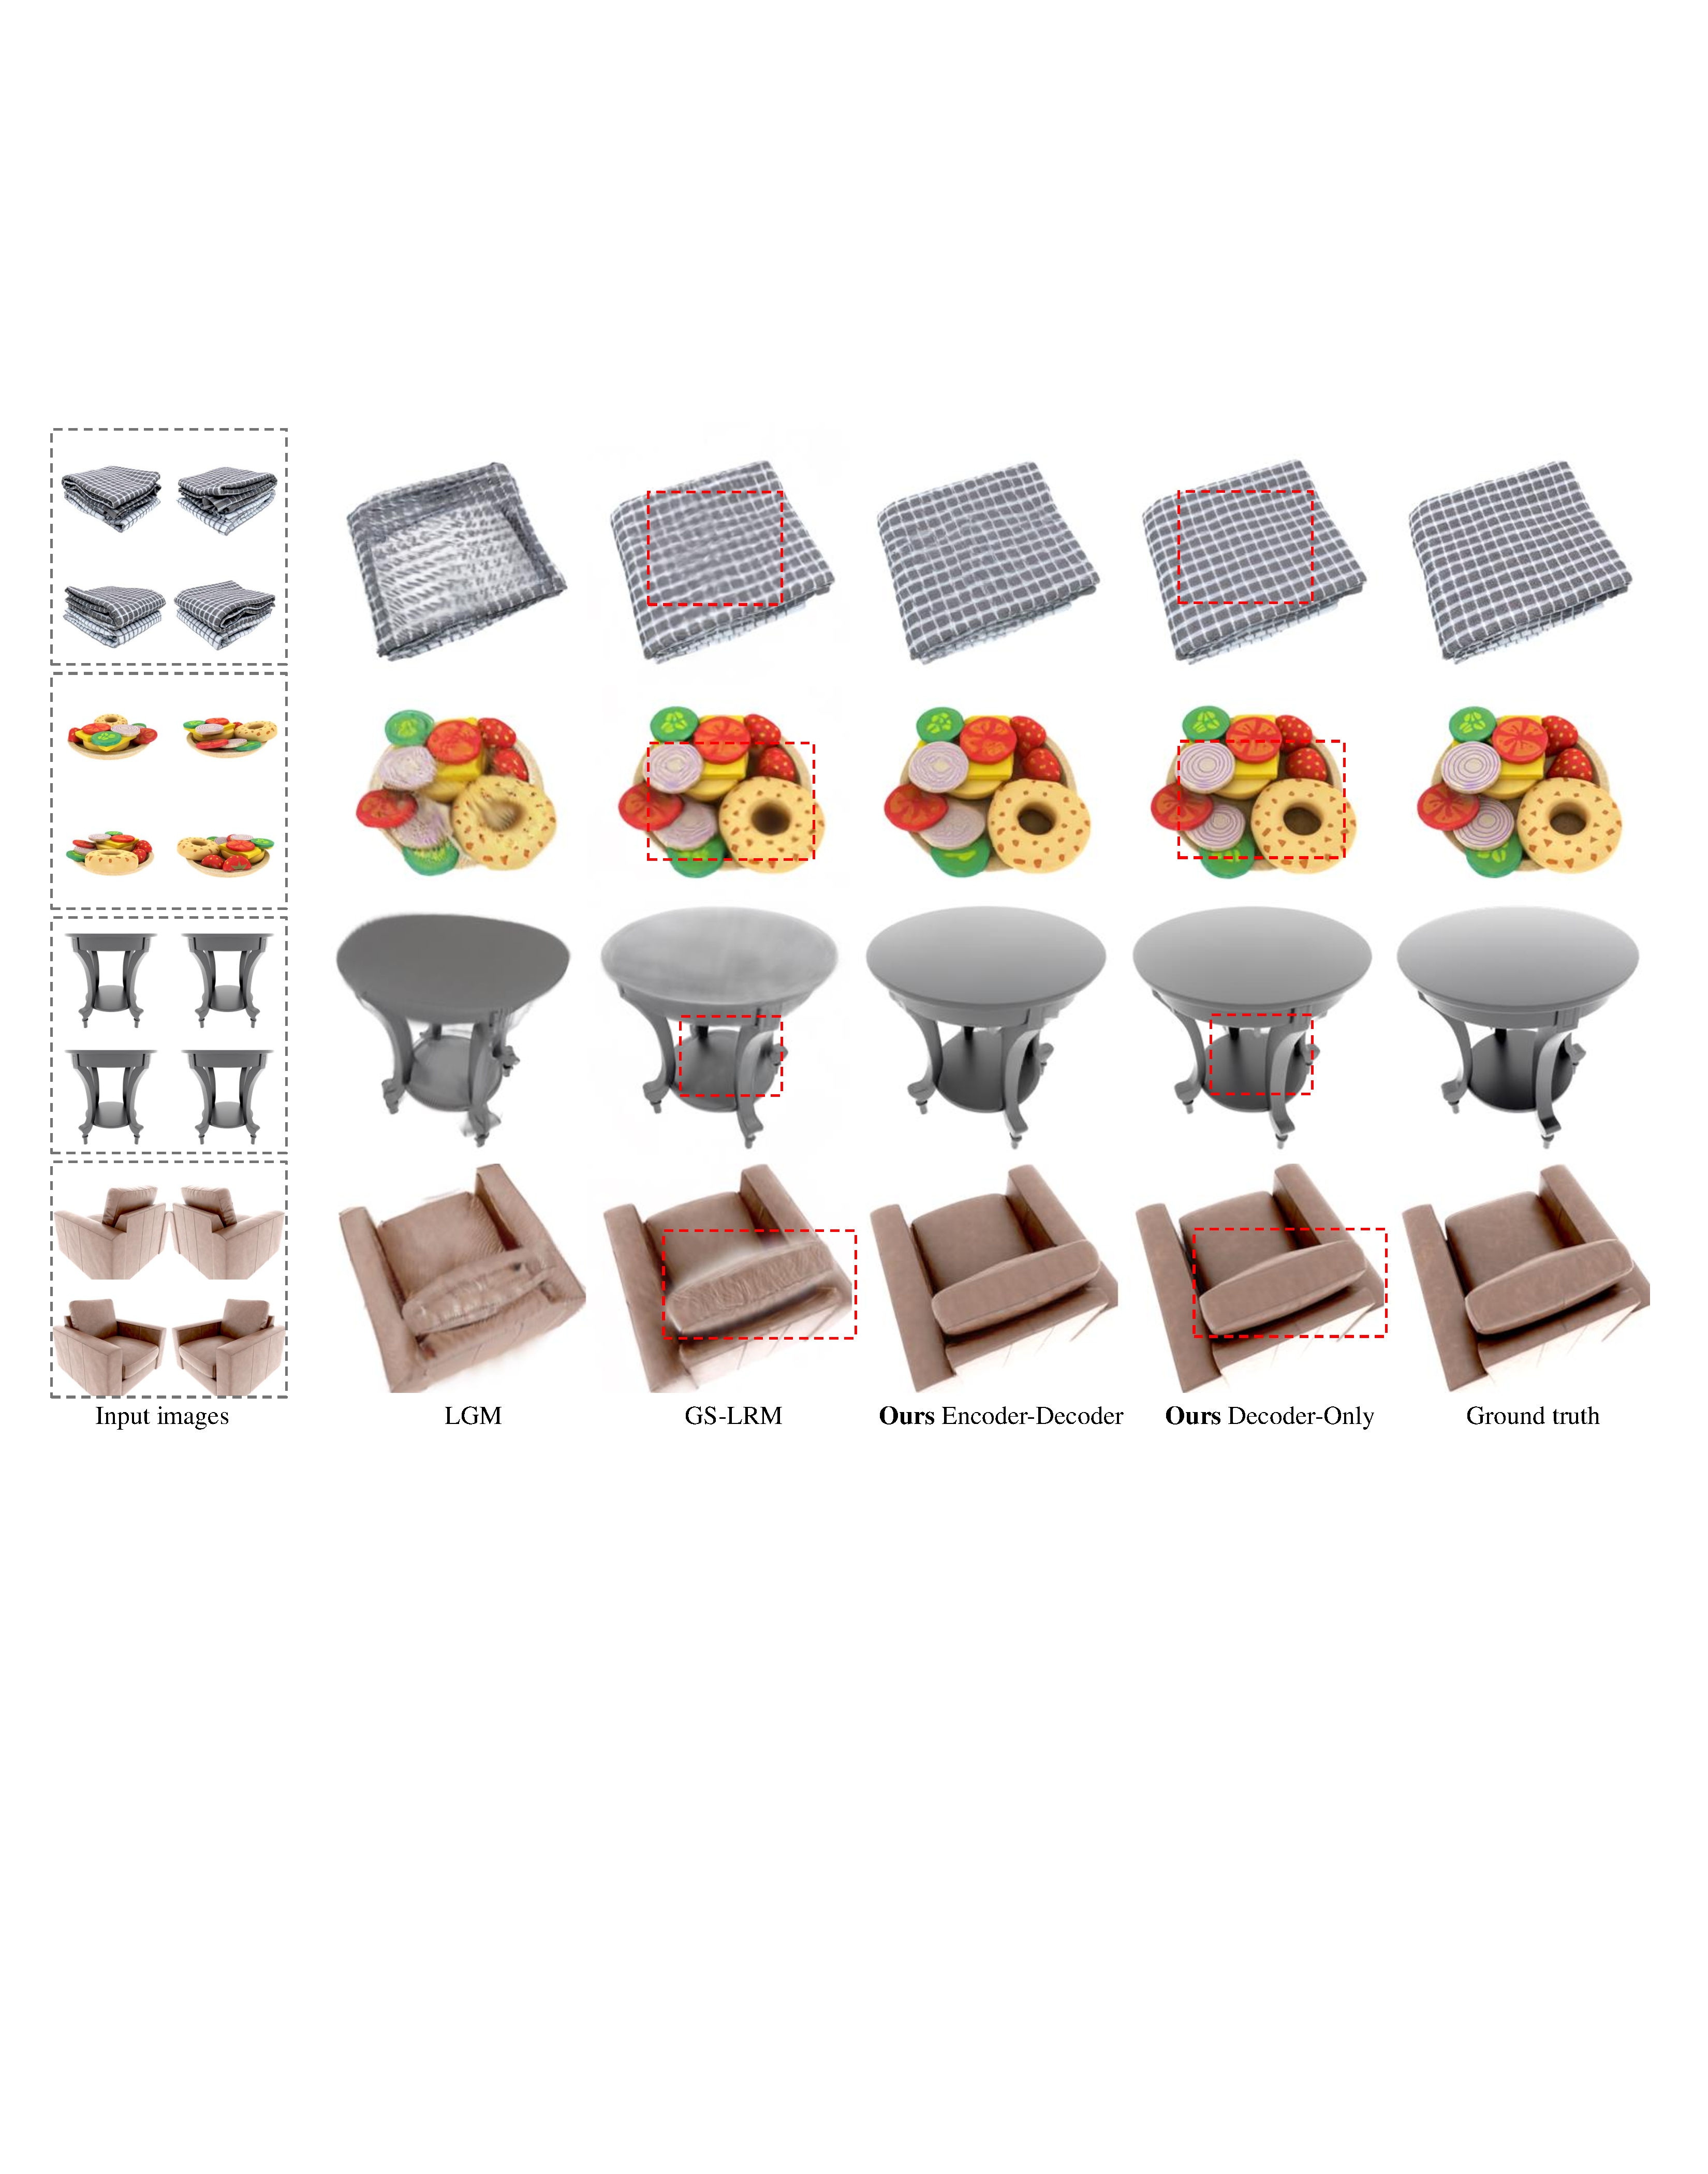
\includegraphics[width=0.95\textwidth]{./figures/object_comparison_256.pdf}
    \vspace{-0.5em}
    \caption{\textbf{Object-level visual comparison at 256 resolution.}
    Comparing with the two baselines: \textit{LGM}\citep{tang2024lgm} and \textit{GS-LRM} (Res-256)~\citep{zhang2024gslrmlargereconstructionmodel}, 
    both our Encoder-Decoder and Decoder-Only models have fewer floater artifacts (last example), and can generate more accurate view-dependent effects (third example). Our Decoder-Only model can better preserve the texture details (first two examples).
    }
    \label{fig:lowres_obj}
    \vspace{-2em}
\end{figure}


\subsection{Detailed model architecture}
\label{appendix:model_diagrams}

\begin{figure}[h]
    \centering
    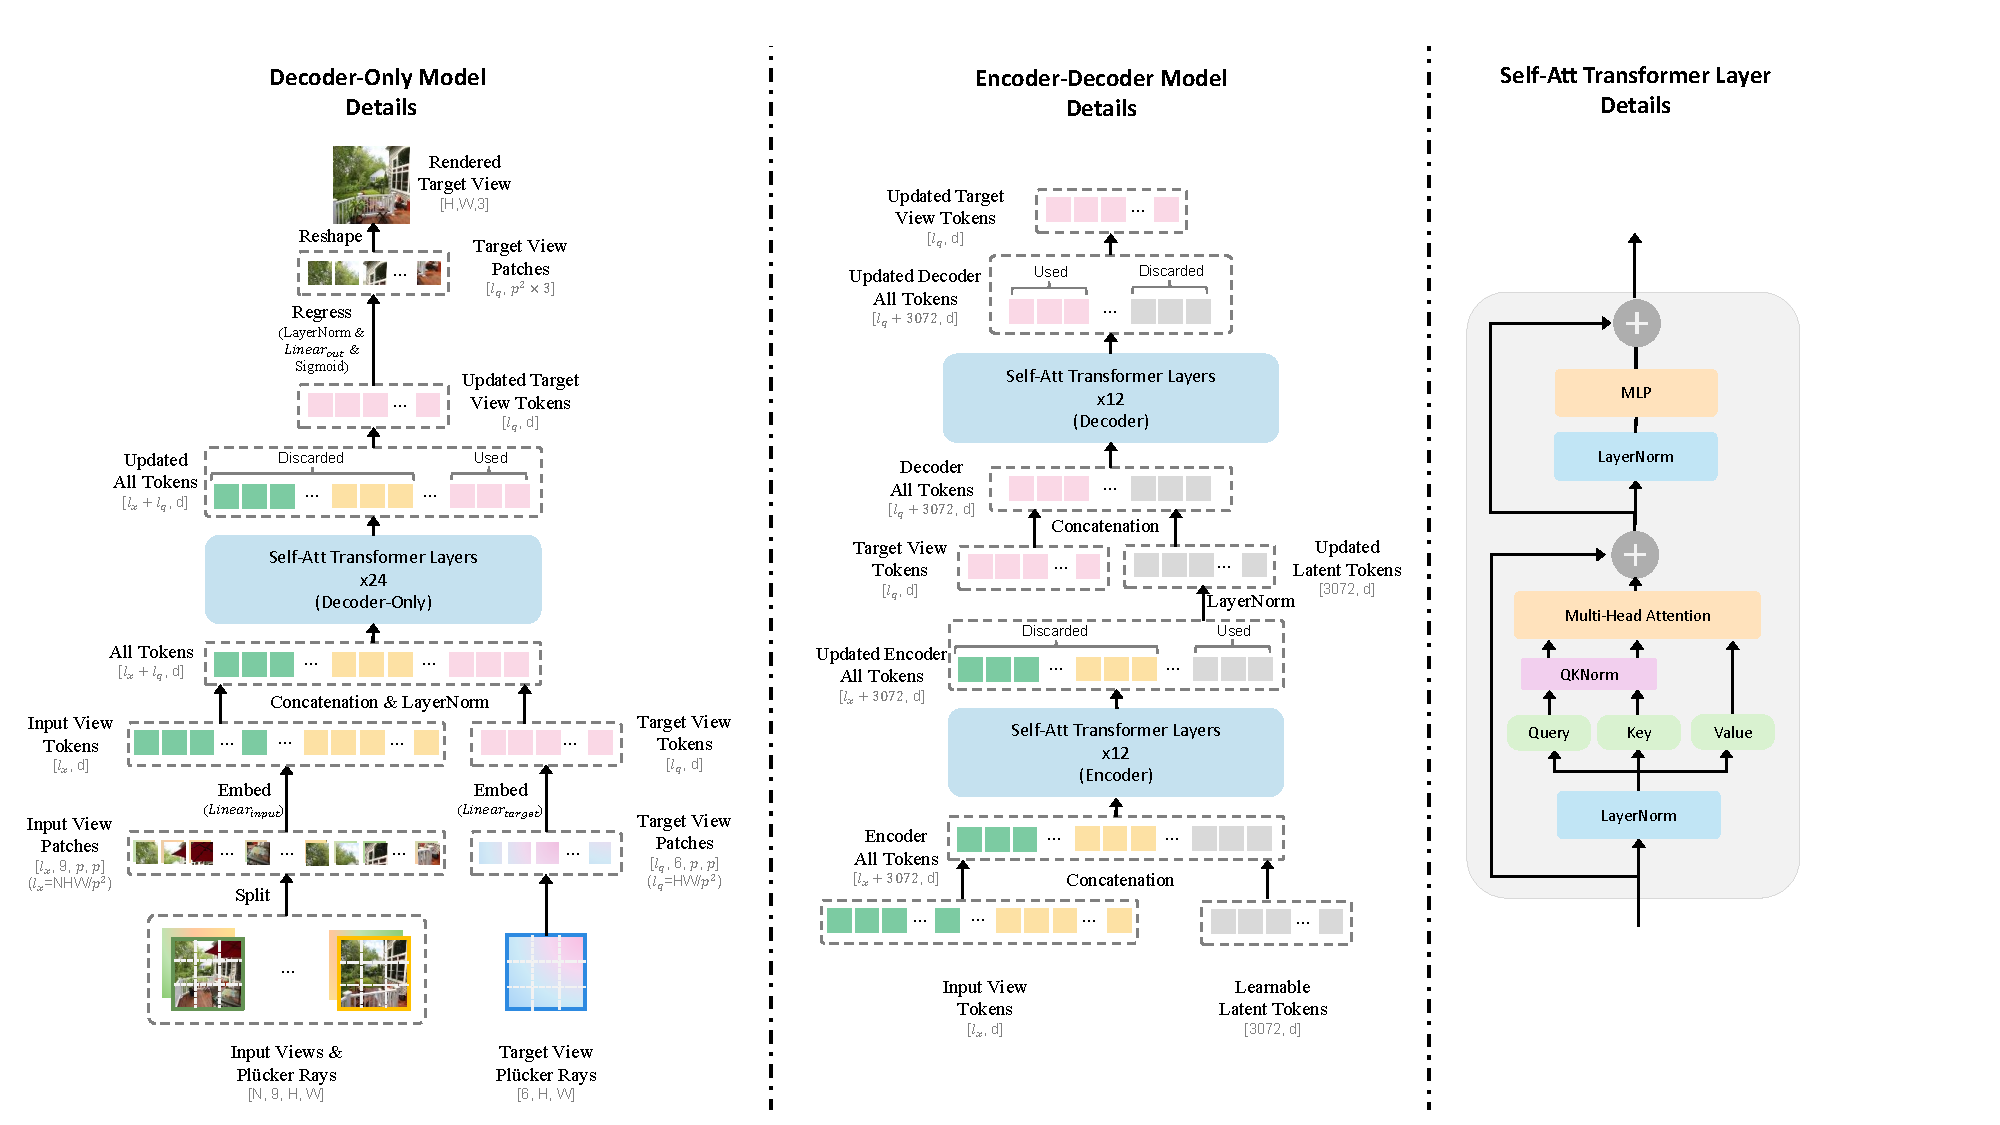
\includegraphics[width=\textwidth]{./figures/method_details.pdf}
    \vspace{-0.5em}
    \caption{\textbf{Model Details.}
    We introduce two architectures: (1) an encoder-decoder LVSM, which
encodes input image tokens into a fixed number of 1D latent tokens, functioning as a fully-learned latent scene representation, and decodes novel-view images from
them; and (2) a decoder-only LVSM, which directly maps input images to novel view outputs, completely eliminating intermediate scene representations. Both models consist of pure self-attention blocks.
    }
    \label{fig:detailed_architecture}
\end{figure}
We have provided a detailed model architecture figure, as shown in Fig.~\ref{fig:detailed_architecture}.

\subsection{Attention mask illustration for different design choices}
In Fig.~\ref{fig:attention_mask}, we visualize the corresponding attention masks for the various design choices discussed in Sec.~\ref{sec: exp_ablation}.

\begin{figure}[h!]
    \centering
    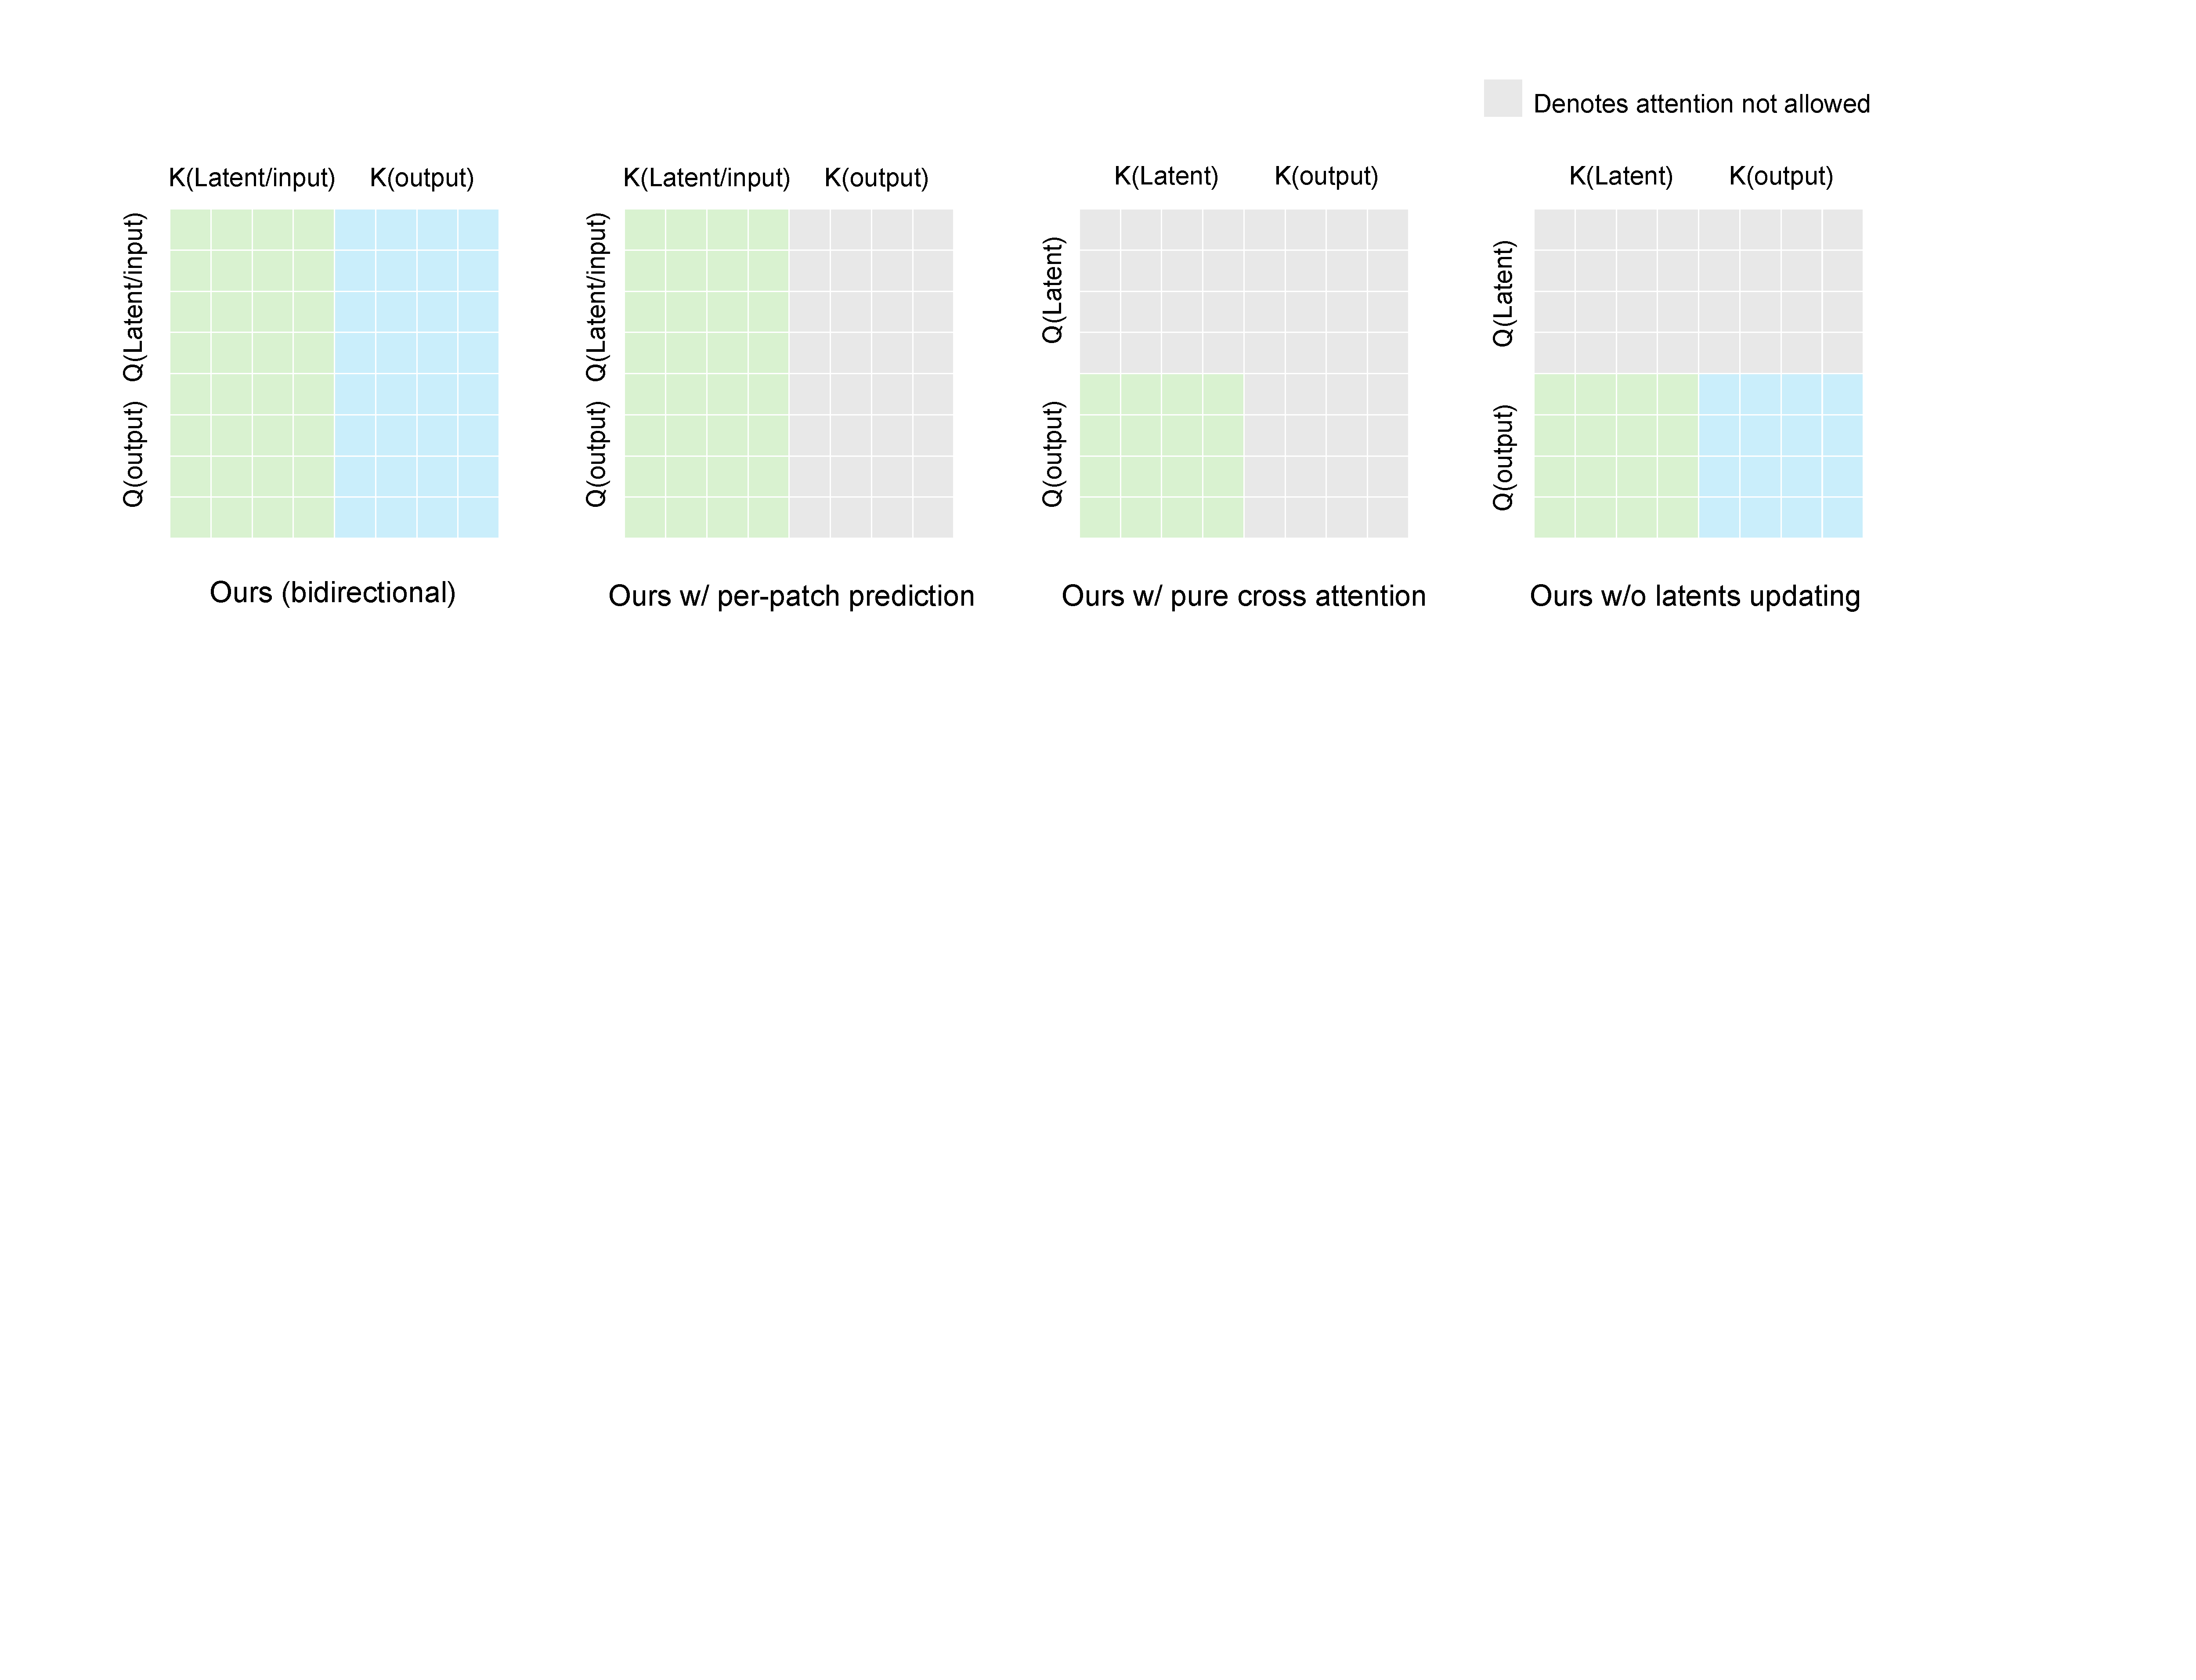
\includegraphics[width=\textwidth]{./figures/attention_mask.pdf}
    \vspace{-2em}
    \caption{\textbf{Attention Mask Visualization.}
    Both our encoder-decoder and decoder-only models employ bidirectional self-attention modules. This figure visualizes the corresponding attention masks for the various design choices discussed in Sec.~\ref{sec: exp_ablation}. (We use green color for the columns of latent/input tokens and blue for the columns of output pixel patch tokens.) In our encoder-decoder architecture, the decoder utilizes pure self-attention, enabling latent tokens and different output target image tokens to jointly attend to each other. Consequently, latent tokens can be updated across transformer layers, while different output patch pixels can also attend to each other for joint updates. As shown in Table~\ref{table: ablation_model_arch}, disabling either the joint updating of output patch pixels (ours w/ per-patch prediction) or the latents' updating (ours w/o latents' updating) significantly degrades performance. Prior work, SRT~\citep{sajjadi2022srt}, eliminates both mechanisms by employing a decoder with pure cross-attention (ours w/ pure cross-att decoder), leading to even worse performance. Similarly, in our decoder-only model, disabling the joint updating of output patch pixels (ours w/ per-patch prediction) also results in a notable performance drop.
    }
    \label{fig:attention_mask}
\end{figure}



\subsection{Discussion of differences with prior generative NVS models}
\label{appendix: diff_from_generative_model}


Motivated by the success of the previous NVS geometry-free approaches~\citep{sitzmann2021lightfieldnetwork,sajjadi2022srt}, and the effectiveness of diffusion models in image-to-image tasks~\citep{saharia2022palette,ramesh2022hierarchical,saharia2022image}, 3DiM~\citep{watson2022novel} explores training image-to-image diffusion models for object-level multi-view rendering to perform novel view synthesis without an explicit 3D representation. 
However, 3DiMs is trained from scratch using limited 3D data~\citep{sitzmann2019scene}, limiting it to category-specific settings and without zero-shot generalization.

The following work Zero-1-to-3~\citep{liu2023zero1to3} adopts a similar pipeline without a 3D representation but fine-tunes its model from a pretrained 2D diffusion model using a larger 3D object dataset~\citep{deitke2023objaverse}, achieving better generalization and higher quality. 
However, Zero-1-to-3’s view synthesis results suffer from inherent multi-view inconsistency because it is a probabilistic model and it generates one target image at a time independently. 

To improve this inconsistency problem, several works~\citep{liu2023syncdreamer, yang2023consistnet, ye2023consistent, tung2024megascenes} integrate additional forms of 3D inductive bias, such as a 3D representation, epipolar attention, etc., into the diffusion denoising process, leading to increased computational cost. 
Other approaches~\citep{li2023instant3d,shi2023zero123plus,shi2023MVDream,long2023wonder3d} predict a single image grid representing (specific) multi-view images with fixed camera pose, sacrificing the ability to control the camera. More recent works, including Free3D~\citep{zheng2024free3d}, EscherNet~\citep{kong2024eschernet}, CAT3D~\citep{gao2024cat3d}, SV3D~\citep{voleti2025sv3d}, and some other video model based work~\citep{wang2024motionctrl, he2024cameractrl, yu2024viewcrafter,yan2024streetcrafterstreetviewsynthesis}, jointly predict multiple target views with accurate camera control while ensuring view consistency by integrating cross-view attention.  However, these methods guarantee consistency only for the finite set of jointly predicted views.

In contrast, our generalizable deterministic models do not possess the same inherent inconsistency issues of probabilistic models. 
As demonstrated in the video results on our project webpage, after being trained on large-scale multi-view data, our models can independently generate each target image with precise camera control while maintaining view consistency---without relying on the cross-view attention mechanisms employed by previous generative models. 
This capability enables our models to generate an unlimited number of consistent views for the observed regions of reconstructed scenes, unlike prior generative models. 
Nonetheless, our deterministic models have their own inherent limitations, i.e., they can't hallucinate unseen regions, which are discussed in Appendix~\ref{appendix: limitation}.



\label{appendix: limitation}


\subsection{Limitations}
\label{appendix: limitation}

Our models are deterministic, and like all prior deterministic approaches~\citep{chen2021mvsnerffastgeneralizableradiance,wang2021ibrnetlearningmultiviewimagebased, sajjadi2022srt, wang2023pflrm,zhang2024gslrmlargereconstructionmodel}, they struggle to produce high-quality results in unseen regions. Previous 3D-based deterministic models typically generate blurry artifacts for those regions due to uncertainty, whereas our model often generates noisy and flickering artifacts with fixed patterns. To illustrate this, we provide video examples of related failure cases on our webpage. Incorporating generative techniques or combining generative methods with our model could help solve this issue, which we leave as a promising future direction.


Additionally, our model's performance degrades when provided with images with aspect ratios and resolutions different from those seen during training. For instance, when trained on $512 \times 512$ images and tested on $512 \times 960$ input images, we observe high-quality novel view synthesis at the center of the output but blurred regions at the horizontal boundaries that extend beyond the training aspect ratio. We hypothesize that this limitation arises because our model is trained on center-cropped images. Specifically, the Pl\"{u}cker ray density is smaller at the boundaries of the image's longer side, and since our model is not trained on such data, it struggles to generalize. Expanding the training dataset to include more diverse image resolutions and aspect ratios could help address this issue.